\chapter{Fabricação e montagem}

\section{CAD}

blabla

\begin{figure}[h]
	\centering
	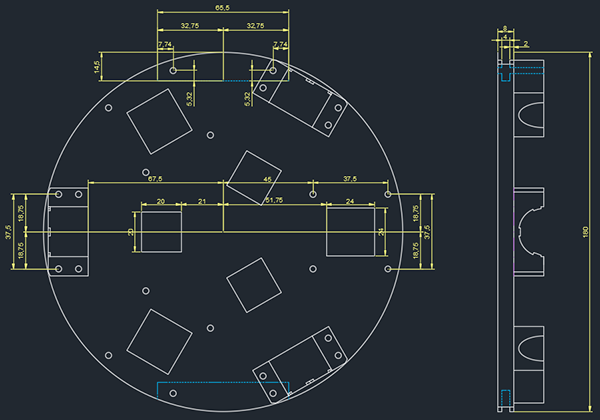
\includegraphics{figures/cad1}
	\caption{Base do robô}
	\label{fig:base_robo}
\end{figure}

\begin{figure}[h]
	\centering
	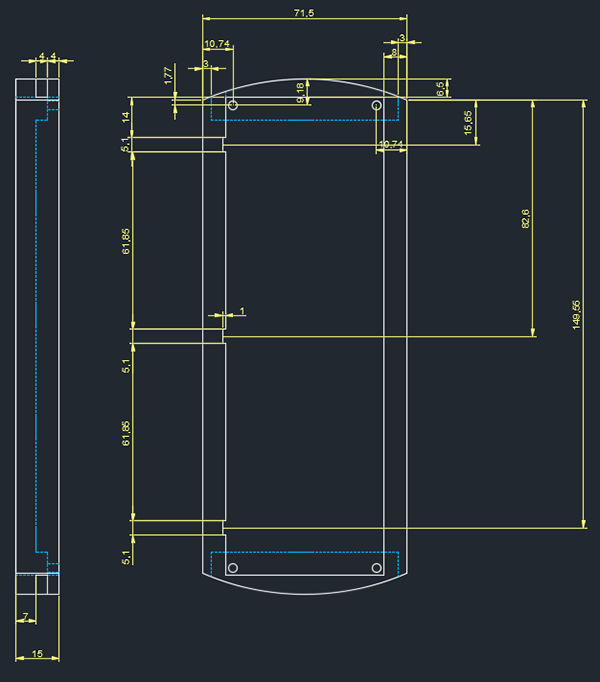
\includegraphics{figures/cad2}
	\caption{Suporte Protoboard}
	\label{fig:suport_protoboard}
\end{figure}

\begin{figure}[h]
	\centering
	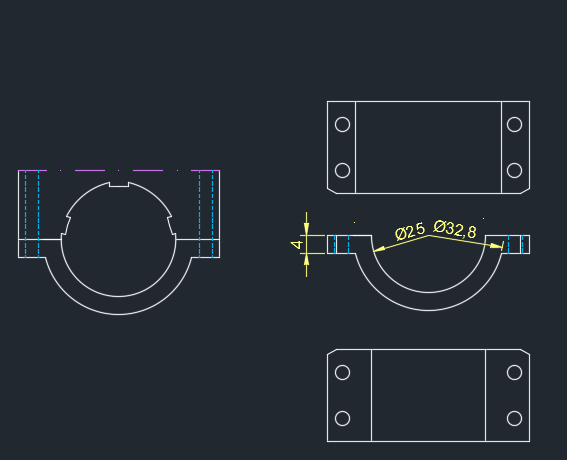
\includegraphics{figures/cad3}
	\caption{Mancais dos Motores - 1}
	\label{fig:mancais}
\end{figure}

\begin{figure}[h]
	\centering
	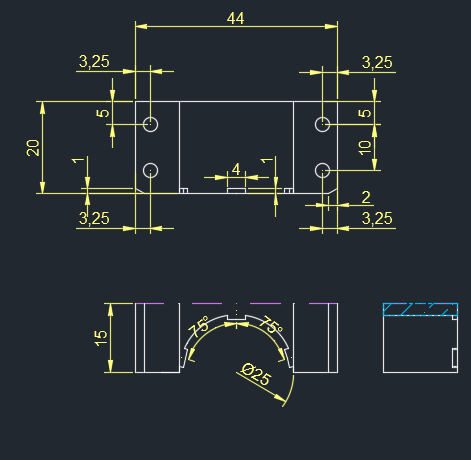
\includegraphics{figures/cad3_2}
	\caption{Mancais dos Motores - 2}
	\label{fig:mancais_2}
\end{figure}

\begin{figure}[h]
	\centering
	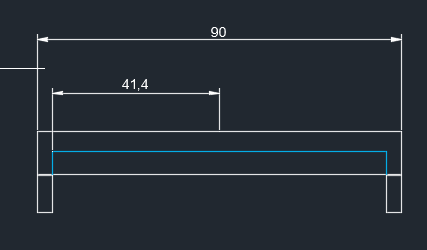
\includegraphics{figures/cad4}
	\caption{peça que conecta o suporte de protoboard e a base - 1}
	\label{fig:peca_juncao}
\end{figure}

\begin{figure}[h]
	\centering
	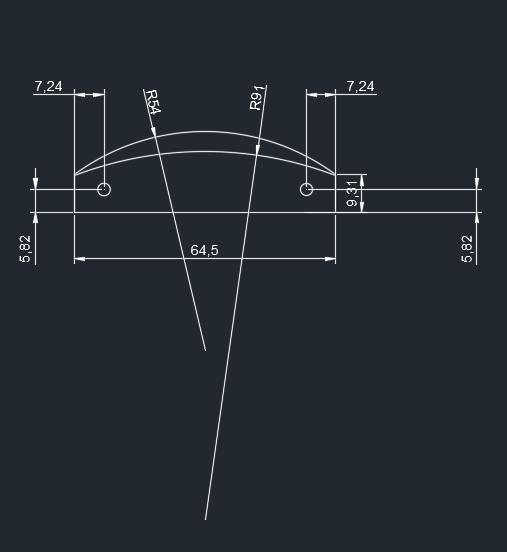
\includegraphics{figures/cad4_2}
	\caption{peça que conecta o suporte de protoboard e a base - 2}
	\label{fig:peca_juncao_2}
\end{figure}



\section{modelagem 3D}

blabla

\begin{figure}[h]
	\centering
	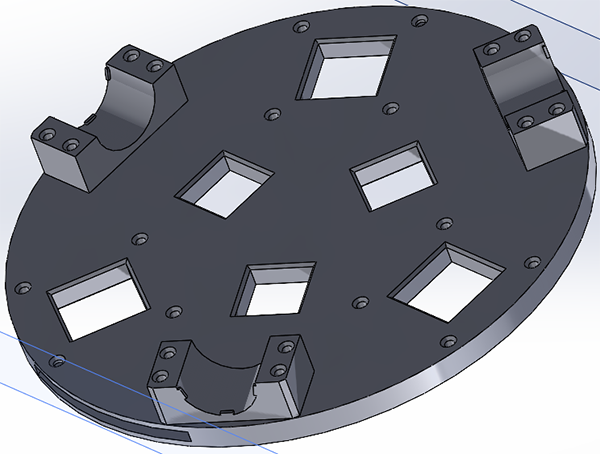
\includegraphics{figures/3d_1}
	\caption{Modelagem 3d da base do robô}
	\label{fig:base_robo_3d}
\end{figure}

\begin{figure}[h]
	\centering
	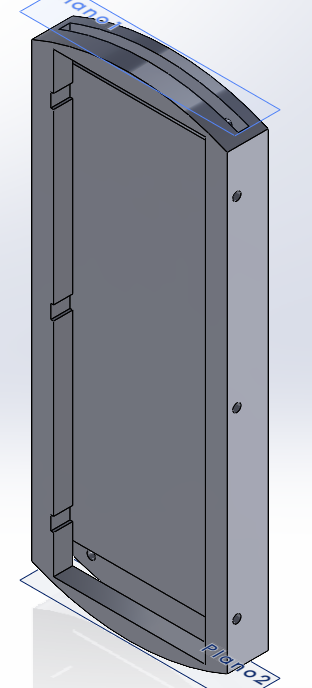
\includegraphics{figures/3d_2}
	\caption{Modelagem 3d do suporte do protoboard}
	\label{fig:suport_protoboard_3d}
\end{figure}

\begin{figure}[h]
	\centering
	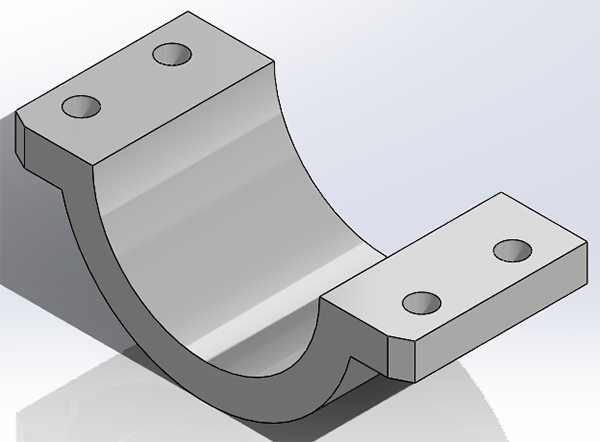
\includegraphics{figures/3d_3}
	\caption{Modelagem 3d dos mancais}
	\label{fig:mancais_3d}
\end{figure}

\begin{figure}[h]
	\centering
	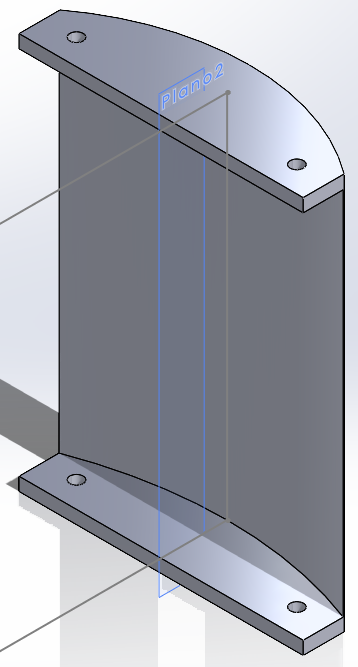
\includegraphics{figures/3d_4}
	\caption{Modelagem 3d peça de junção}
	\label{fig:peca_juncao_3d}
\end{figure}


\section{Impressão e montagem}

\begin{figure}[h]
	\centering
	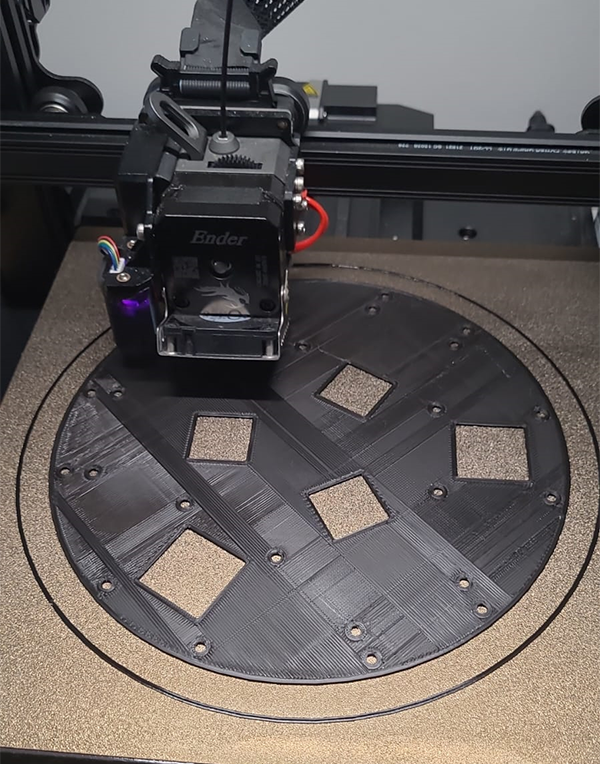
\includegraphics{figures/impressao}
	\caption{Impressão das peças}
	\label{fig:impressao}
\end{figure}

\begin{figure}[h]
	\centering
	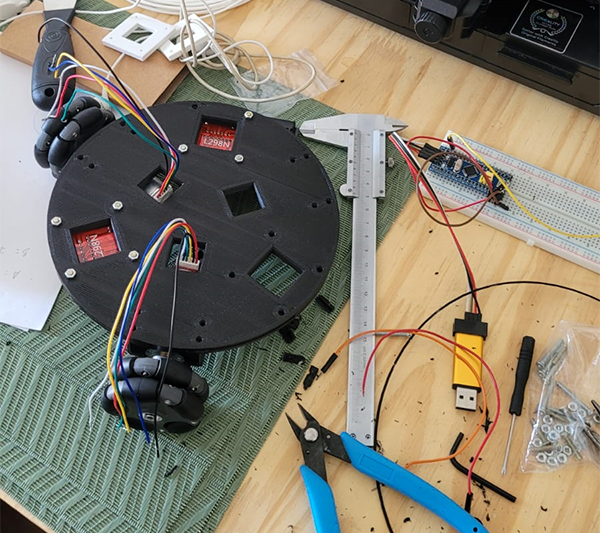
\includegraphics{figures/montagem_1}
	\caption{Montagem 1}
	\label{fig:montagem}
\end{figure}

\begin{figure}[h]
	\centering
	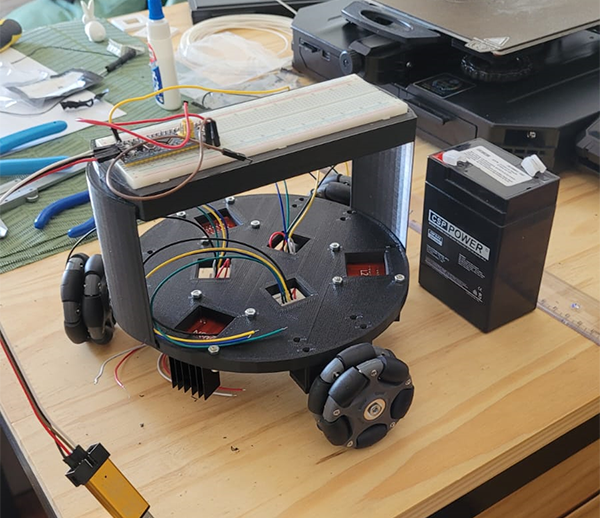
\includegraphics{figures/montagem_2}
	\caption{Montagem 2}
	\label{fig:montagem_2}
\end{figure}

\begin{figure}[h]
	\centering
	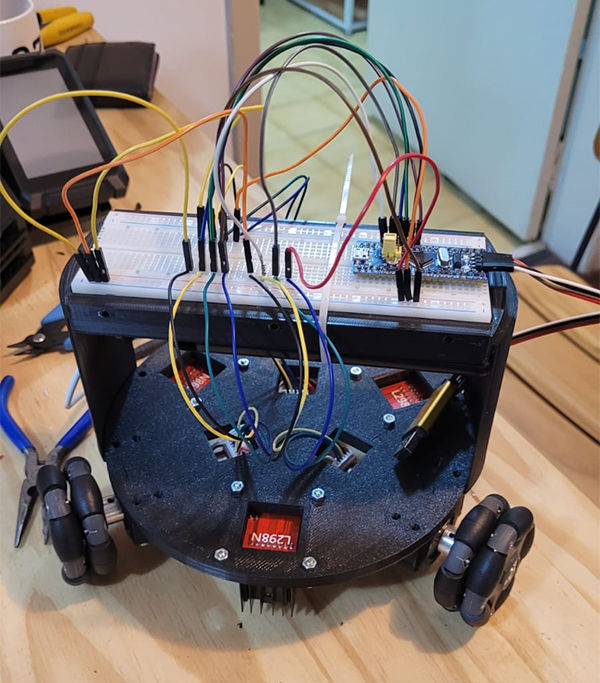
\includegraphics{figures/montagem_3}
	\caption{Montagem 3}
	\label{fig:montagem_3}
\end{figure}


\begin{figure}[h]
	\centering
	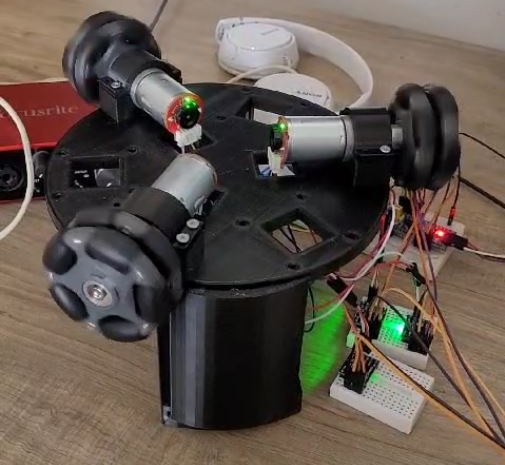
\includegraphics{figures/montagem_4}
	\caption{Testes dos motores}
	\label{fig:montagem_4}
\end{figure}
